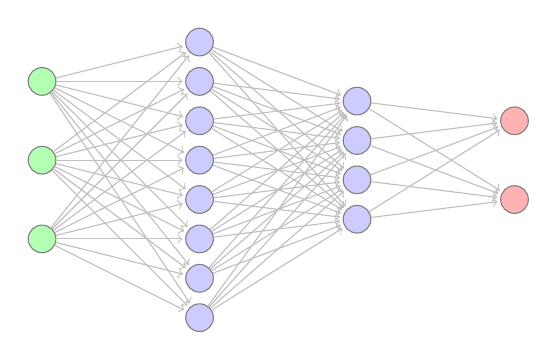
\begin{tikzpicture}
    \tikzstyle{neuron} = [circle, draw=black!50, fill=blue!20, minimum size=10pt, inner sep=0pt];
    \tikzstyle{input} = [neuron, fill=green!30]
    \tikzstyle{output} = [neuron, fill=red!30]
    \tikzstyle{marrow} = [gray!50,->,shorten >=1pt];

    \foreach \x in {1,...,3}
        \node[input] (I-\x) at (-2,\x - 1.5) {};

    \foreach \y in {1,...,8}
        \node[neuron] (H-\y) at (0,\y*0.5 - 2) {};

    \foreach \r in {1,...,4}
        \node[neuron] (S-\r) at (2,\r*0.5 - 0.75) {};

    \foreach \z in {1,...,2}
        \node[output] (O-\z) at (4,\z - 1) {};
    
    \foreach \x in {1,...,3}
        \foreach \y in {1,...,8}
            \draw[marrow] (I-\x) edge (H-\y);

    \foreach \y in {1,...,8}
        \foreach \r in {1,...,4}
            \draw[marrow] (H-\y) edge (S-\r);
    
    \foreach \r in {1,...,4}
        \foreach \z in {1,...,2}
            \draw[marrow] (S-\r) edge (O-\z);

\end{tikzpicture}